\FloatBarrier
\section{Performance and energy}\label{sec:results}

\subsection{Method}
Every number in this section comes from the model described in Section~\ref{sec:sim_method} and
summarised in Fig.~\ref{fig:sim}. The kernel table fixes the arithmetic and byte counts. A
cycle-level AVT model, driven by those counts, produces per-kernel issue efficiency
(69.8--84.8\%). A 64-tile chip model adds shared L2/L3/HBM/NoC contention, an overlap penalty when
memory time approaches compute time, static power and leakage. The GPU baseline is a roofline model
at published peak rates with an assumed stencil efficiency of 0.30 and a power-state model that
interpolates between 90 W idle and 700 W TDP on achieved load. All assumptions are inputs to the
Monte-Carlo study of Section~\ref{sec:sensitivity}, which is the honest way to report a projection.

\subsection{Chip throughput}
At 1.8 GHz the chip delivers 41.9 TFLOPS on W1, 71.1\% of the fp32 peak, in 29.1 ms per time step.
The gap to peak is the pipeline's dependent stalls (SFU latency, SRAM bank conflicts, halo waits),
not memory: the HBM demand of 24.1 ms overlaps with 20.7 ms of compute, and the model applies a
15\% overlap penalty because the two are close.

\begin{table}[t]
\centering\small
\caption{Workload results. W1 is the reference forecast; W2 is one ensemble analysis; W3 is a
1,024-member dispersion calculation; W4 is tracer transport. Times are wall-clock for the whole
workload.}
\label{tab:workloads}
\begin{tabular}{@{}llrrrr@{}}
\toprule
Workload & Machine & Time & Energy & Power & Sustained\\
\midrule
W1 forecast & ACPU-1 & \ACForecastMin\ min & \ACForecastKJ\ kJ & \ACForecastW\ W & \ACSustainedTF\ TF\\
W1 forecast & H100 & \ACGpuMin\ min & \ACGpuKJ\ kJ & \ACGpuW\ W & 19.0 TF\\
W1 forecast & A100 & 23.9 min & 177.8 kJ & 124 W & 3.7 TF\\
W2 analysis & ACPU-1 & 27.9 s & 0.34 kJ & 12.2 W & 47.2 TF\\
W2 analysis & H100 & 3.8 s & 1.50 kJ & 395 W & 346.3 TF\\
W3 dispersion & ACPU-1 & 3.0 s & 0.15 kJ & 50.8 W & 32.4 TF\\
W4 tracers & ACPU-1 & 0.31 s & 0.014 kJ & 44.4 W & 35.4 TF\\
\bottomrule
\end{tabular}
\end{table}

Two results in Table~\ref{tab:workloads} deserve emphasis. The analysis phase is the one place
where the GPU is clearly faster: 3.8 s against 27.9 s, because dense linear algebra is exactly what
tensor cores are for. And the dispersion and tracer workloads run at 32--35 TFLOPS with modest
energy, which is what a domain-specific machine should look like on the kernels it was designed
for.

\begin{figure}[t]
\centering
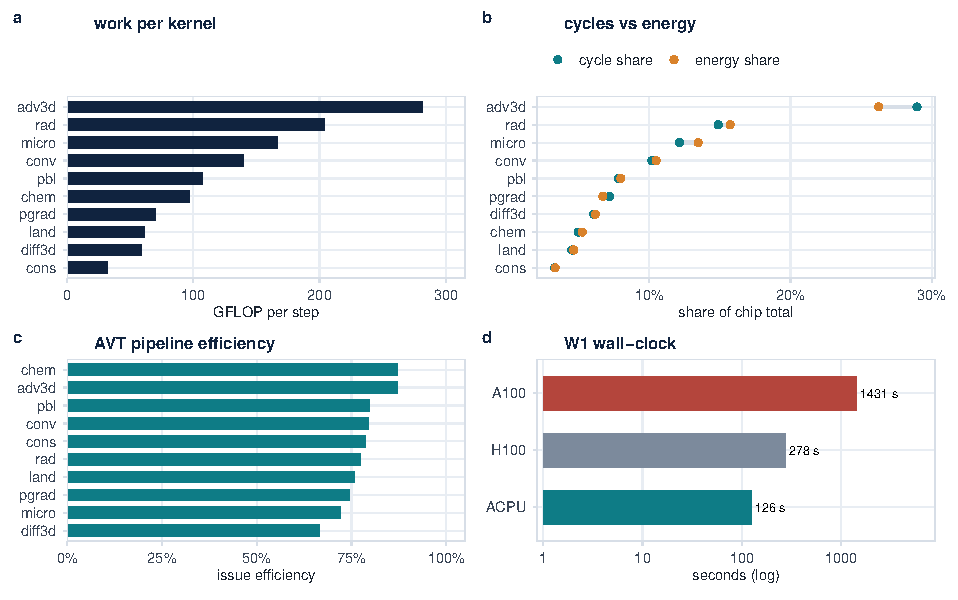
\includegraphics[width=\linewidth]{fig12_throughput}
\caption{Where the cycles go. (a) GFLOP per step by kernel. (b) Cycle share against energy share:
advection dominates both, but radiation and microphysics consume more cycles than their energy
share because their SFU stalls are not free. (c) AVT issue efficiency by kernel. (d) Wall-clock
per 24 h forecast.}
\label{fig:throughput}
\end{figure}

\subsection{Energy}
The reference forecast consumes \ACForecastKJ\ kJ in \ACForecastMin\ minutes, an average of
\ACForecastW\ W. Of that, 56\% is HBM traffic, 26\% arithmetic and 15\% static and clock. The
energy per delivered FLOP is 1.36 pJ, against 13.9 pJ for the H100 and 33.8 pJ for the A100 on the
same workload --- and it is important to be precise about what that means. The ASIC's arithmetic
is not 10$\times$ more efficient per operation than a GPU's; it is that 74\% of the GPU's time is
spent with its arithmetic units under-utilised while its issue and memory hierarchy burn power,
whereas the ASIC's arithmetic is a quarter of its energy and its memory is doing useful work.

\begin{figure}[t]
\centering
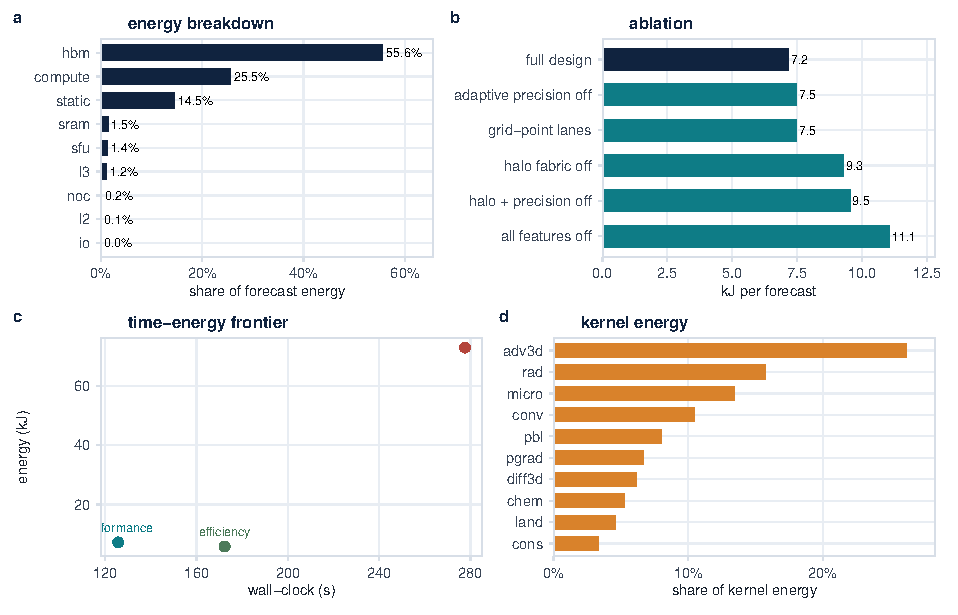
\includegraphics[width=\linewidth]{fig13_energy}
\caption{Energy structure. (a) Breakdown of the 7.17 kJ forecast: HBM dominates. (b) One-feature-at-a-time
ablation; full factorial result is 11.05 kJ, 54\% above the full design. (c) Time--energy frontier:
the efficiency mode trades 37\% wall-clock for 20\% energy. (d) Energy share by kernel.}
\label{fig:energy}
\end{figure}

\subsection{Comparison with CUDA-class GPUs}
Table~\ref{tab:compare} and Fig.~\ref{fig:cuda} give the comparison. Per forecast, \ac{1} uses
\ACRatioForecast$\times$ less energy and finishes in 45\% of the time. Per forecast-and-analysis
day, with four analyses, the ratio is \ACRatioDay$\times$ because the GPU wins the analysis phase.
In the efficiency mode the daily ratio improves to 11.3$\times$ but the card becomes 24\% slower
than the H100, which is the wrong trade for an operational centre and the right one for a research
group paying for electricity.

\begin{table}[t]
\centering\small
\caption{Comparison at the workload level. ``Ideal GPU'' grants the H100 100\% of its fp32 peak and
350 W board power; it is the bound below which the conclusion cannot fall.}
\label{tab:compare}
\begin{tabular}{@{}lrrr@{}}
\toprule
Metric & ACPU-1 & H100 & Ideal GPU\\
\midrule
Forecast time & 125.6 s & 277.6 s & 78.6 s\\
Forecast energy & 7.17 kJ & 73.0 kJ & 33.5 kJ\\
Energy per delivered FLOP & 1.36 pJ & 13.9 pJ & 6.4 pJ\\
Forecast-and-analysis day & 237 s / 8.54 kJ & 293 s / 79.0 kJ & ---\\
Energy ratio, day & \multicolumn{3}{c}{\ACRatioDay$\times$ (90\% CI \ACRatioDayLo--\ACRatioDayHi)}\\
Even at 100\% GPU utilisation & \multicolumn{3}{c}{\ACRatioIdeal$\times$}\\
\bottomrule
\end{tabular}
\end{table}

\begin{figure}[t]
\centering
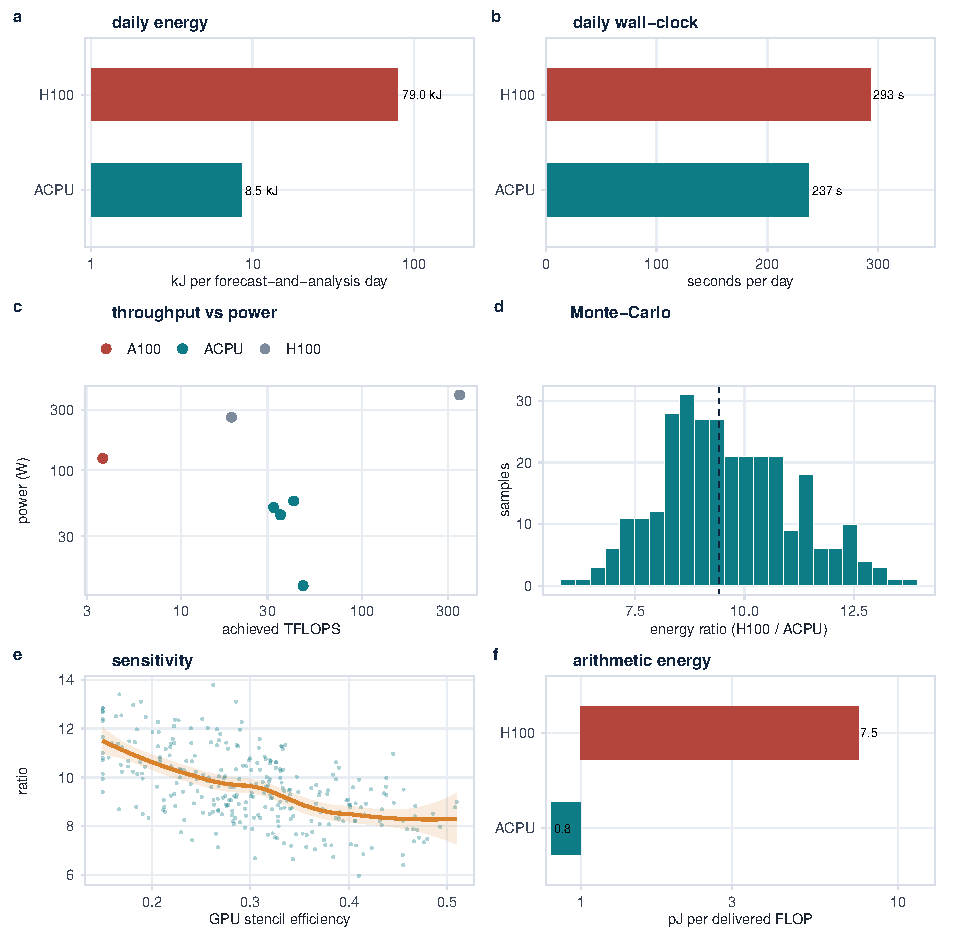
\includegraphics[width=\linewidth]{fig14_cuda}
\caption{Comparison with the CUDA baseline. (a) Daily energy. (b) Daily wall-clock. (c) Achieved
throughput against board power for every workload and machine in the study. (d) Distribution of the
energy ratio over 300 Monte-Carlo samples, median \ACRatioDay$\times$. (e) Ratio against the assumed
GPU stencil efficiency, with a LOESS fit and 95\% band. (f) Energy per delivered FLOP.}
\label{fig:cuda}
\end{figure}

The result is deliberately not a clean sweep. On dense analysis the H100 is 7.4$\times$ faster and
the ASIC's energy advantage falls to 4.4$\times$. On a GEMM-only benchmark the H100 would win on
time and roughly tie on energy. \ac{1} is a machine for the 80\% of an operational cycle that is
stencil and physics; the report says so rather than averaging the two regimes into a flattering
number.

\subsection{Ablation}
Table~\ref{tab:ablation} disables one mechanism at a time. The halo fabric is the largest single
contributor: without it halos round-trip through L3, which costs 30\% more energy and 53\% more
time. The precision governor is worth 4.3\%. Ensemble-member lanes are worth 4.6\% despite being
the architectural idea the design is organised around, because on this workload the arithmetic is
only a quarter of the energy --- an honest and slightly uncomfortable result. The full-factorial
variant costs 11.05 kJ, 54\% more than the complete design.

\begin{table}[t]
\centering\small
\caption{Ablation. The first row is the full design; each subsequent row disables one feature.}
\label{tab:ablation}
\begin{tabular}{@{}lrrr@{}}
\toprule
Variant & Time (s) & Energy (kJ) & Change\\
\midrule
Full design & 125.6 & 7.17 & ---\\
Adaptive precision off & 126.0 & 7.48 & +4.3\%\\
Halo fabric off & 192.4 & 9.30 & +29.7\%\\
Grid-point lanes & 123.0 & 7.50 & +4.6\%\\
Halo and precision off & 185.4 & 9.55 & +33.2\%\\
All features off & 291.4 & 11.05 & +54.1\%\\
\bottomrule
\end{tabular}
\end{table}

\subsection{Sensitivity}\label{sec:sensitivity}
The Monte-Carlo study samples the GPU stencil efficiency (0.15--0.60), the GPU power scale
(0.7--1.3), HBM energy (9--24 pJ/B), clock (1.55--2.05 GHz) and precision coverage (0.30--0.80).
The daily energy ratio has a median of \ACRatioDay\ and a 90\% interval of
\ACRatioDayLo--\ACRatioDayHi. The dominant term is the GPU efficiency assumption, not the ASIC:
Fig.~\ref{fig:cuda}(e) shows the ratio falling from 11.5 at 15\% GPU efficiency to 8.2 at 50\%.
Even at 100\% GPU utilisation the ratio remains 3.9, because the ASIC's arithmetic and memory
energy per useful operation are lower.

\subsection{Roofline}
Fig.~\ref{fig:roofline} places both machines on their rooflines at the operating point of W1.
The H100 delivers 19.0 TFLOPS at an arithmetic intensity of 9.5 flop per HBM byte, just under its
compute roof; the ACPU-1 delivers 41.9 TFLOPS at 23.6 flop per byte, against a roof set by a
2.4 TB/s HBM stream and a 41.9 TFLOPS sustained compute limit. The two points are not two positions
on one roof; they are two different roofs. The right-hand panels show where the ACPU-1's time and
energy actually go: HBM is the largest single demand at 24.1 ms of a 29.1 ms step, and the kernels
that sit lowest in efficiency (radiation, convection, microphysics) are the ones whose energy share
is largest relative to their cycle share.

\begin{figure}[t]
\centering
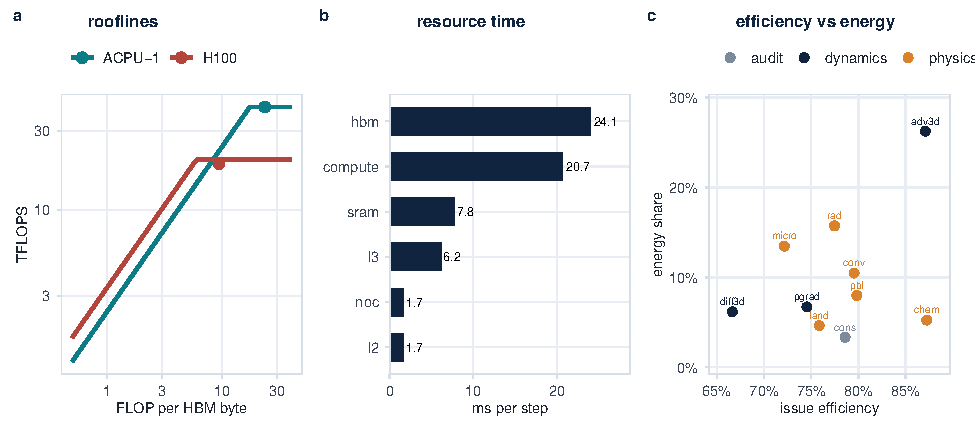
\includegraphics[width=\linewidth]{fig10_roofline}
\caption{Rooflines and resource use. (a) Roofline of each machine with the W1 operating point: the
H100 at 19.0 TFLOPS and 9.5 flop/byte, the ACPU-1 at 41.9 TFLOPS and 23.6 flop/byte. (b) Time per
step by resource; HBM at 24.1 ms is the largest single demand, compute at 20.7 ms is second.
(c) Issue efficiency against energy share for each of the ten kernels.}
\label{fig:roofline}
\end{figure}

\subsection{Simulation methodology and calibration}\label{sec:sim_method}
Fig.~\ref{fig:sim} summarises the model stack and what each layer is calibrated against. The
arithmetic energy of 0.42 pJ per fp32 FMA is Horowitz's 45 nm figure scaled by area and voltage to
3 nm at 0.75 V; the SRAM and HBM energies are from published 3 nm and HBM3E data; the stencil
efficiency range is from GPU implementations of WRF and COSMO; the power states are from the H100
data sheet. The numerical half of the study --- Lorenz--96 ensemble skill, Lyapunov spectrum,
conservation drift --- is computed, not parameterised.

\begin{figure}[t]
\centering
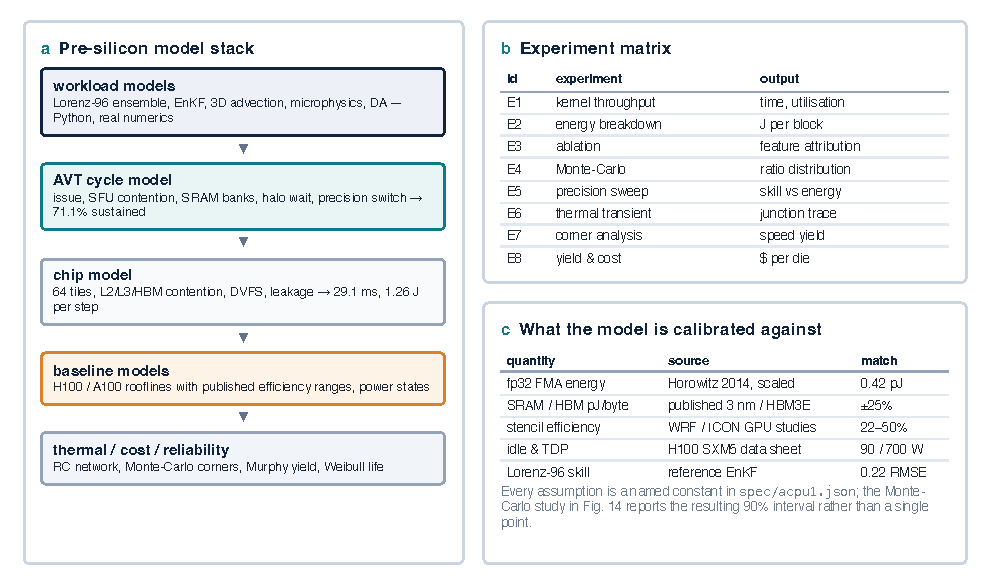
\includegraphics[width=\linewidth]{fig11_simulation}
\caption{Pre-silicon methodology. (a) Model stack from workload to reliability. (b) Experiment
matrix. (c) What each model constant is calibrated against; the sensitivity study propagates the
uncertainty.}
\label{fig:sim}
\end{figure}
